\documentclass[tikz, border=5mm]{standalone}
\usetikzlibrary {arrows.meta}

\definecolor{ovalcolor}{RGB}{180,180,180}
\definecolor{arrowcolor}{RGB}{0,0,0}
\usepackage{xcolor}
\colorlet{myred}{red!80!black}
\colorlet{myblue}{blue!80!black}
\colorlet{mybluee}{myblue!80!black}
\colorlet{mygreen}{green!60!black}
\colorlet{myorange}{orange!70!red!60!black}
\colorlet{mydarkred}{red!30!black}
\colorlet{mydarkblue}{blue!40!black}
\colorlet{mydarkgreen}{green!30!black}

\begin{document}
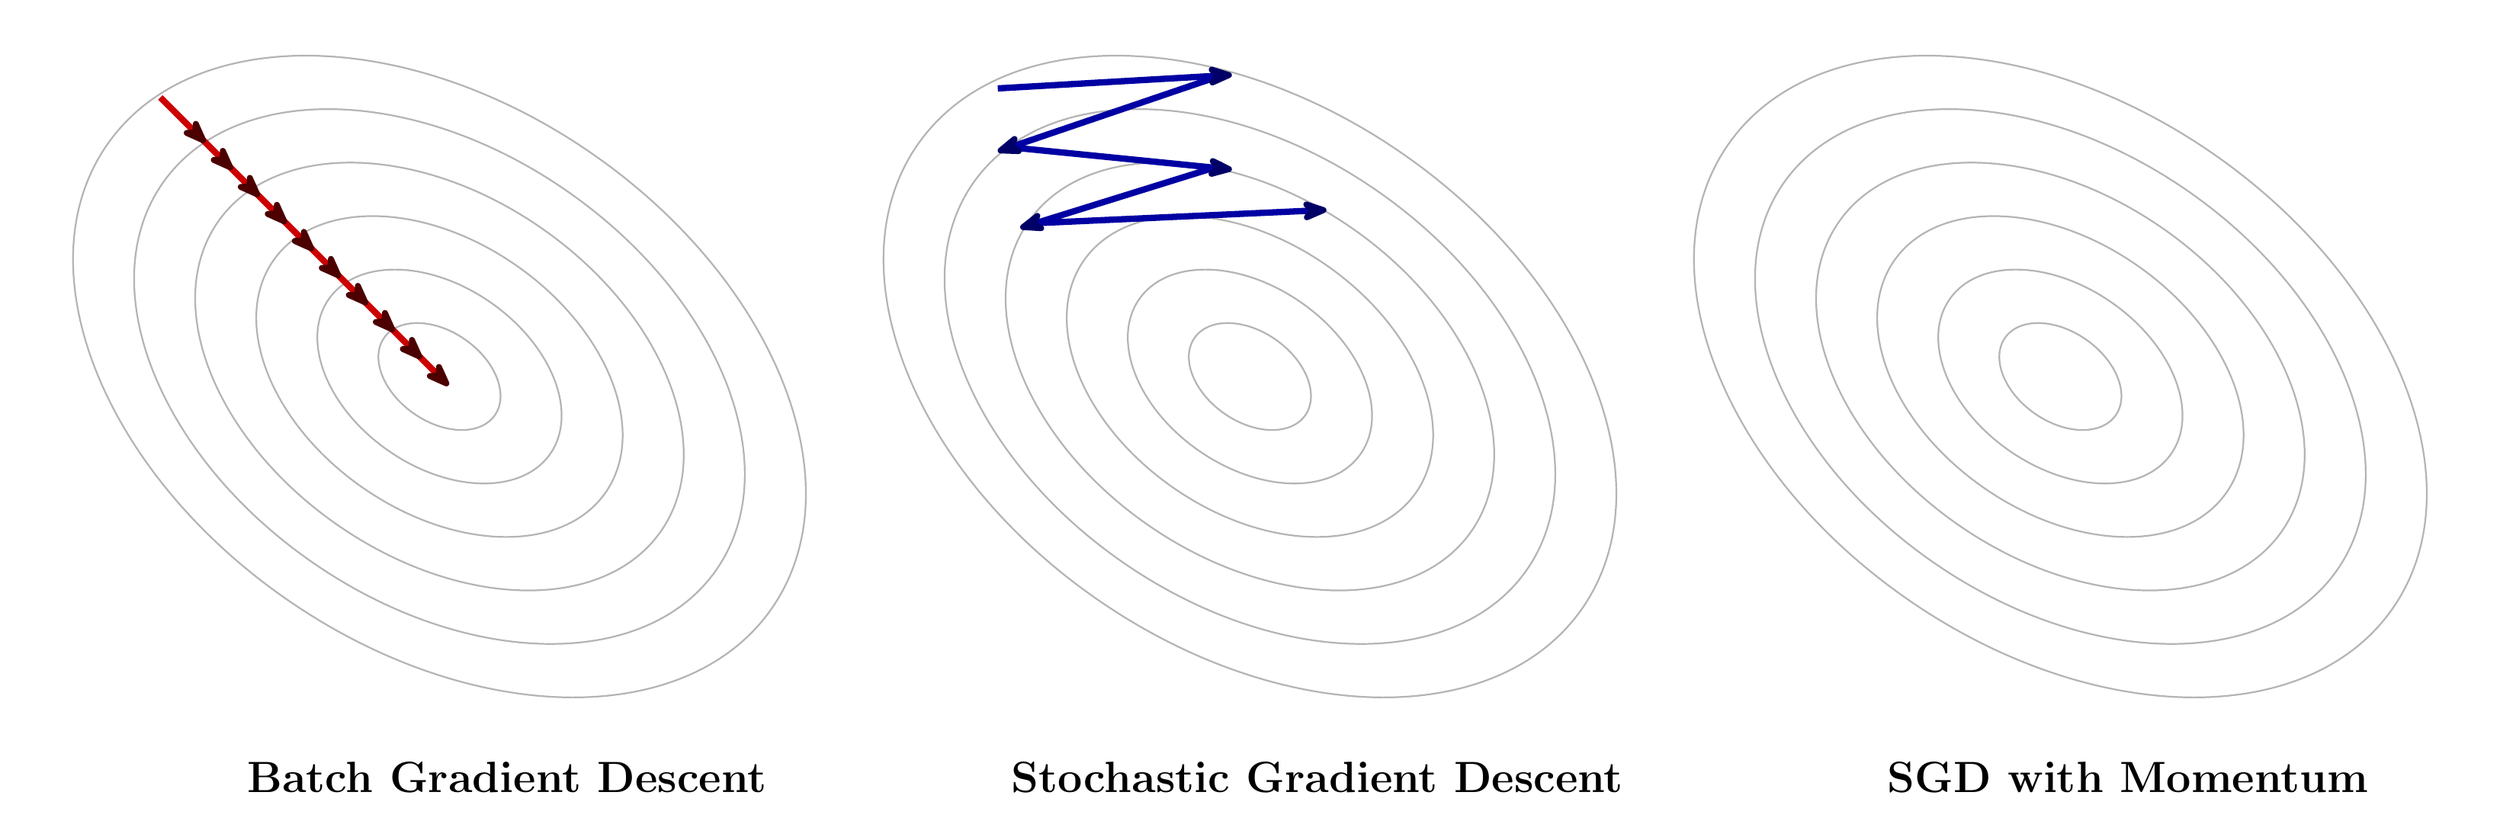
\begin{tikzpicture}[>=stealth, scale=0.75]

\begin{scope}[shift={(-6,0)}]
    \foreach \r in {1, 2, 3, 4, 5, 6}{
        \draw[ovalcolor, thick, rotate=145] (0,0) ellipse ({\r*1.5} and {\r});
    }
\end{scope}

\begin{scope}[shift={(12,0)}]
\foreach \r in {1, 2, 3, 4, 5, 6}{
        \draw[ovalcolor, thick, rotate=145] (0,0) ellipse ({\r*1.5} and {\r});
    }
\end{scope}

\begin{scope}[shift={(30,0)}]
\foreach \r in {1, 2, 3, 4, 5, 6}{
        \draw[ovalcolor, thick, rotate=145] (0,0) ellipse ({\r*1.5} and {\r});
    }
\end{scope}

\node at (-4.5,-8.9) {\huge\textbf{Batch Gradient Descent}};
\node at (13.5,-8.9) {\huge\textbf{Stochastic Gradient Descent}};
\node at (31.5,-8.9) {\huge\textbf{SGD with Momentum}};

\draw [line width=3pt, myred, arrows = {-Stealth[round,color=mydarkred]}] (-6.6,0.6) -- (-5.8,-0.2);
\draw [line width=3pt, myred, arrows = {-Stealth[round,color=mydarkred]}] (-7.2,1.2) -- (-6.4,0.4);
\draw [line width=3pt, myred, arrows = {-Stealth[round,color=mydarkred]}] (-7.8,1.8) -- (-7,1);
\draw [line width=3pt, myred, arrows = {-Stealth[round,color=mydarkred]}] (-8.4,2.4) -- (-7.6,1.6);
\draw [line width=3pt, myred, arrows = {-Stealth[round,color=mydarkred]}] (-9,3) -- (-8.2,2.2);
\draw [line width=3pt, myred, arrows = {-Stealth[round,color=mydarkred]}] (-9.6,3.6) -- (-8.8,2.8);
\draw [line width=3pt, myred, arrows = {-Stealth[round,color=mydarkred]}] (-10.2,4.2) -- (-9.4,3.4);
\draw [line width=3pt, myred, arrows = {-Stealth[round,color=mydarkred]}] (-10.8,4.8) -- (-10,4);
\draw [line width=3pt, myred, arrows = {-Stealth[round,color=mydarkred]}] (-11.4,5.4) -- (-10.6,4.6);
\draw [line width=3pt, myred, arrows = {-Stealth[round,color=mydarkred]}] (-12.2,6.2) -- (-11.2,5.2);


% \draw [line width=3pt, mybluee, arrows = {-Stealth[round,color=mydarkblue]}] (13.6,3.6) -- (6.5,2.5);
\draw [line width=3pt, mybluee, arrows = {-Stealth[round,color=mydarkblue]}] (7.1,3.4) -- (13.7,3.7);
\draw [line width=3pt, mybluee, arrows = {-Stealth[round,color=mydarkblue]}] (11.4,4.7) -- (6.9,3.3);
\draw [line width=3pt, mybluee, arrows = {-Stealth[round,color=mydarkblue]}] (6.6,5.1) -- (11.6,4.6);
\draw [line width=3pt, mybluee, arrows = {-Stealth[round,color=mydarkblue]}] (11.4,6.7) -- (6.4,5);
\draw [line width=3pt, mybluee, arrows = {-Stealth[round,color=mydarkblue]}] (6.4,6.4) -- (11.6,6.7);
\end{tikzpicture}
\end{document}
